\documentclass{bioinfo}
\usepackage{url}

\copyrightyear{}
\pubyear{}

\begin{document}
\firstpage{1}

\title[short Title]{QuickBundles as a method for tractography simplification}
\author[Sample {et~al}]{First Author\,$^{1,*}$, Co-Author\,$^{2}$ and Co-Author\,$^2$\footnote{to whom correspondence should be addressed}}
\address{$^{1}$Department of XXXXXXX, Address XXXX etc.\\
$^{2}$Department of XXXXXXXX, Address XXXX etc.}

\history{}

\editor{}

\maketitle

\begin{abstract}

\section{}
Text Text Text  Text Text Text Text Text Text Text Text
Text  Text Text Text Text Text Text Text Text Text  Text Text Text Text Text Text Text Text Text  Text Text Text Text Text Text Text Text Text  Text Text Text Text Text Text Text Text Text  Text Text Text Text Text Text Text Text Text  Text Text Text Text Text Text  Text Text Text Text Text Text Text Text Text  Text Text Text Text Text Text Text Text Text  Text Text Text Text Text Text Text Text Text  Text Text Text Text Text Text Text  Text Text Text Text Text Text Text Text Text  Text Text Text Text Text Text Text Text Text  Text Text Text Text Text Text Text Text Text  Text

\section{Keywords:} Text Text Text Text Text Text  Text Text Text Text Text Text Text Text Text  Text Text Text
\end{abstract}


\section{Introduction}

Text Text Text Text Text Text  Text Text Text Text Text Text Text Text Text  Text Text Text Text Text Text. \textbf{Figure \ref{fig:01}} shows that the above method  Text Text Text Text  Text Text Text Text Text Text  Text Text.  \citep{Bag01} wants to know about text follows.

\begin{equation}
\sum x+ y =Z\label{eq:01}
\end{equation}


\begin{methods}
\section{Material \& Methods}

Text Text Text Text Text Text  Text Text Text Text Text Text Text Text Text  Text Text Text Text Text Text. \textbf{Figure\ref{fig:02}} shows that the above method  Text Text Text Text  Text Text Text Text Text Text  Text Text.  \citealp{Boffelli03} might want to know about  text text text text
Text Text Text Text Text Text  Text Text Text Text Text Text Text Text Text  Text Text Text Text Text Text. \textbf{Figure\ref{fig:02}} shows that the above method  Text Text Text Text  Text Text Text Text Text Text  Text Text.  \citealp{Boffelli03} might want to know about  text text text text
Text Text Text Text Text Text  Text Text Text Text Text Text Text Text Text  Text Text Text Text Text Text.\textbf{Figure\ref{fig:02}} shows that the above method  Text Text Text Text  Text Text Text Text Text Text  Text Text.  \citealp{Boffelli03} might want to know about  text text text text

\begin{itemize}
\item for bulleted list, use itemize
\item for bulleted list, use itemize
\item for bulleted list, use itemize
\end{itemize}



Text Text Text Text Text Text  Text Text Text Text Text Text Text Text Text  Text Text Text Text Text Text.\textbf{Figure\ref{fig:02}} shows that the above method  Text Text Text Text  Text Text Text Text Text Text  Text Text.  \citealp{Boffelli03} might want to know about  text text text text
Text Text Text Text Text Text  Text Text Text Text Text Text Text Text Text  Text Text Text Text Text Text.\textbf{Figure\ref{fig:02}} shows that the above method  Text Text Text Text  Text Text Text Text Text Text  Text Text.  \citealp{Boffelli03} might want to know about  text text text text
Text Text Text Text Text Text  Text Text Text Text Text Text Text Text Text  Text. For more information, check out the {website$^{}$}\footnote{\url{http://www.math.uiuc.edu/~hildebr/tex}} Text Text Text Text Text.\textbf{Figure\ref{fig:02}} shows that the above method  Text Text Text Text  Text Text Text Text Text Text  Text Text.  \citealp{Boffelli03} might want to know about  text text text text
Text Text Text Text Text Text  Text Text Text Text Text Text Text Text Text  Text Text Text Text Text Text. \textbf{Figure\ref{fig:02}} shows that the above method  Text Text Text Text  Text Text Text Text Text Text  Text Text.  \citealp{Boffelli03} might want to know about  text text text text
Text Text Text Text Text Text  Text Text Text Text Text Text Text Text Text  Text Text Text Text Text Text.

Text Text Text Text Text Text  Text Text Text Text Text Text Text Text Text  Text Text Text Text Text Text. \textbf{Figure\ref{fig:02}} shows that the above method  Text Text Text Text  Text Text Text Text Text Text  Text Text.  \citealp{Boffelli03} might want to know about  text text text text
Text Text Text Text Text Text  Text Text Text Text Text Text Text Text Text  Text Text Text Text Text Text. \textbf{Figure\ref{fig:02}} shows that the above method  Text Text Text Text  Text Text Text Text Text Text  Text Text.  \citealp{Boffelli03} might want to know about  text text text text
Text Text Text Text Text Text  Text Text Text Text Text Text Text Text Text  Text Text Text Text Text Text. \textbf{Figure\ref{fig:02}} shows that the above method  Text Text Text Text  Text Text Text Text Text Text  Text Text.  \citealp{Boffelli03} might want to know about  text text text text



Text Text Text Text Text Text  Text Text Text Text Text Text Text Text Text  Text Text Text Text Text Text. \textbf{Figure\ref{fig:02}} shows that the above method  Text Text Text Text  Text Text Text Text Text Text  Text Text.  \citealp{Boffelli03} might want to know about  text text text text
Text Text Text Text Text Text  Text Text Text Text Text Text Text Text Text  Text Text Text Text Text Text. \textbf{Figure\ref{fig:02}} shows that the above method  Text Text Text Text  Text Text Text Text Text Text  Text Text.  \citealp{Boffelli03} might want to know about  text text text text
Text Text Text Text Text Text  Text Text Text Text Text Text Text Text Text  Text Text Text Text Text Text. \textbf{Figure\ref{fig:02}} shows that the above method  Text Text Text Text  Text Text Text Text Text Text  Text Text.  \citealp{Boffelli03} might want to know about  text text text text.


Text Text Text Text Text Text  Text Text Text Text Text Text Text Text Text  Text Text Text Text Text Text. \textbf{Figure\ref{fig:02}} shows that the above method  Text Text Text Text  Text Text Text Text Text Text  Text Text.  \citealp{Boffelli03} might want to know about  text text text text
Text Text Text Text Text Text  Text Text Text Text Text Text Text Text Text  Text Text Text Text Text Text. \textbf{Figure\ref{fig:02}} shows that the above method  Text Text Text Text  Text Text Text Text Text Text  Text Text.  \citealp{Boffelli03} might want to know about  text text text text
Text Text Text Text Text Text  Text Text Text Text Text Text Text Text Text  Text Text Text Text Text Text. \textbf{Figure\ref{fig:02}} shows that the above method  Text Text Text Text  Text Text Text Text Text Text  Text Text.  \citealp{Boffelli03} might want to know about  text text text text



\begin{table}[!t]
\processtable{This is table caption\label{Tab:01}}
{\begin{tabular}{llll}\toprule
head1 & head2 & head3 & head4\\\midrule
row1 & row1 & row1 & row1\\
row2 & row2 & row2 & row2\\
row3 & row3 & row3 & row3\\
row4 & row4 & row4 & row4\\\botrule
\end{tabular}}{This is a footnote}
\end{table}

\end{methods}

\begin{figure*}[htp]%figure1
\centerline{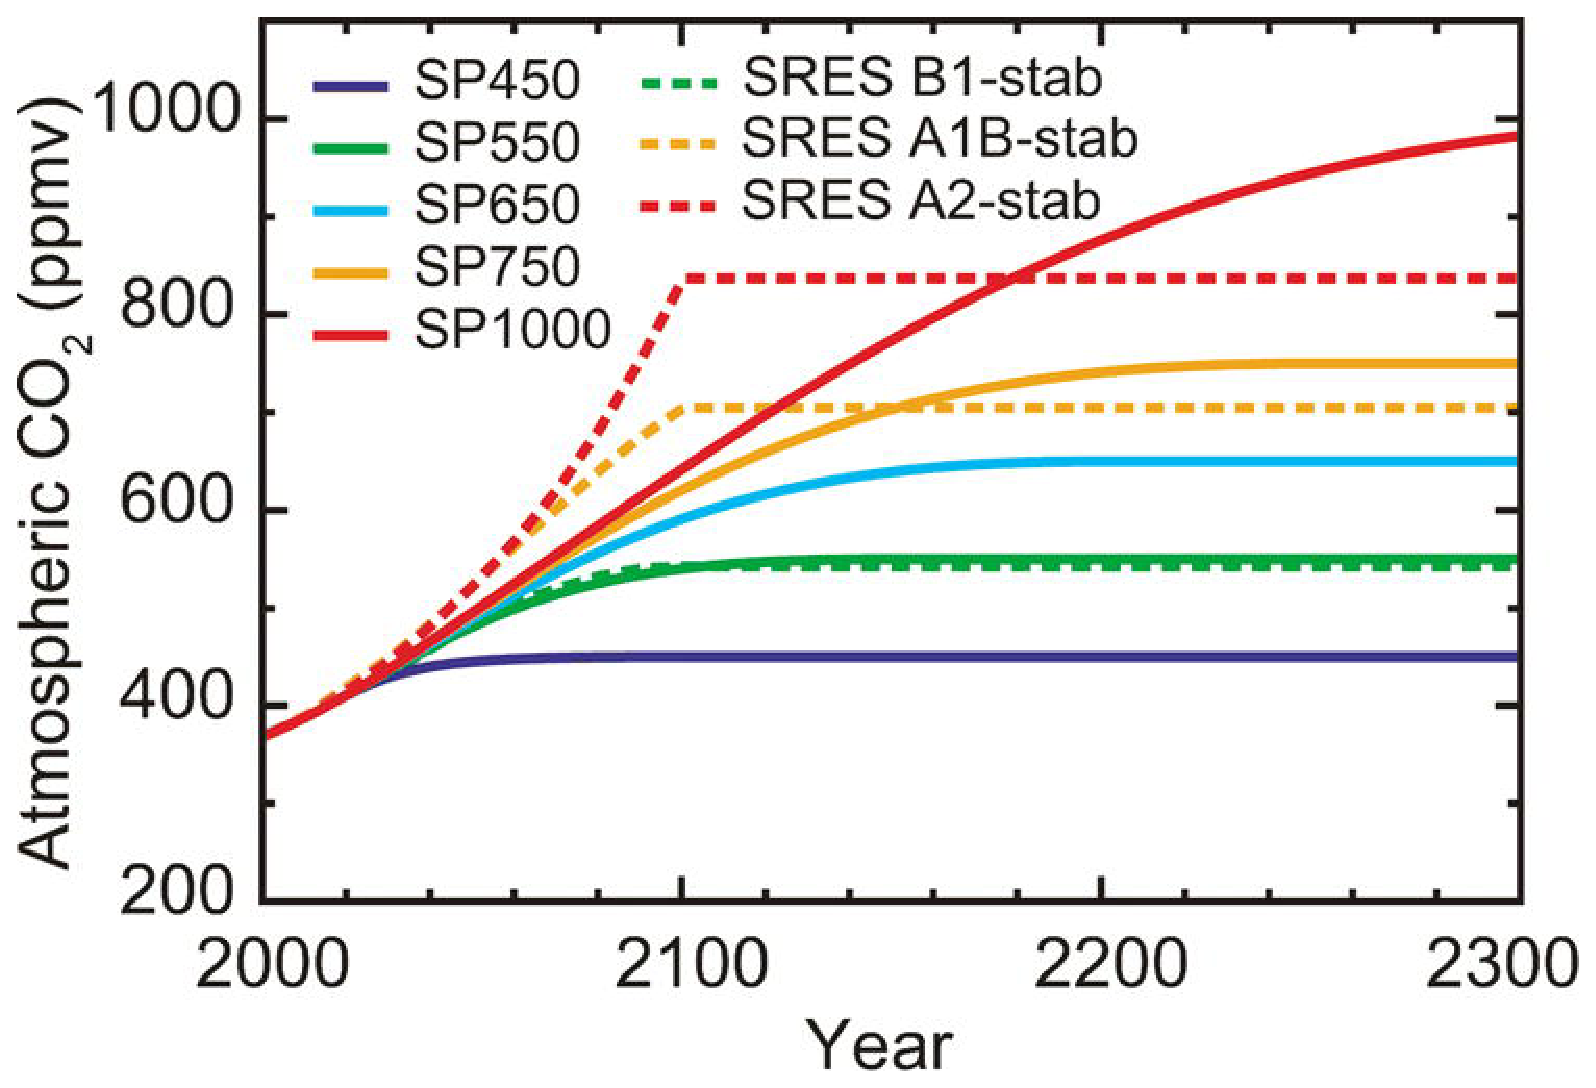
\includegraphics[width=38pc,angle=0]{./figures/figure01.eps}}
\caption{Enter the caption for your figure here.  Repeat as
  necessary for each of your figures. Create a figures directory and
  place all figures in that directory.}\label{fig:01}
\end{figure*}

\begin{figure}[htp]%figure2
\centerline{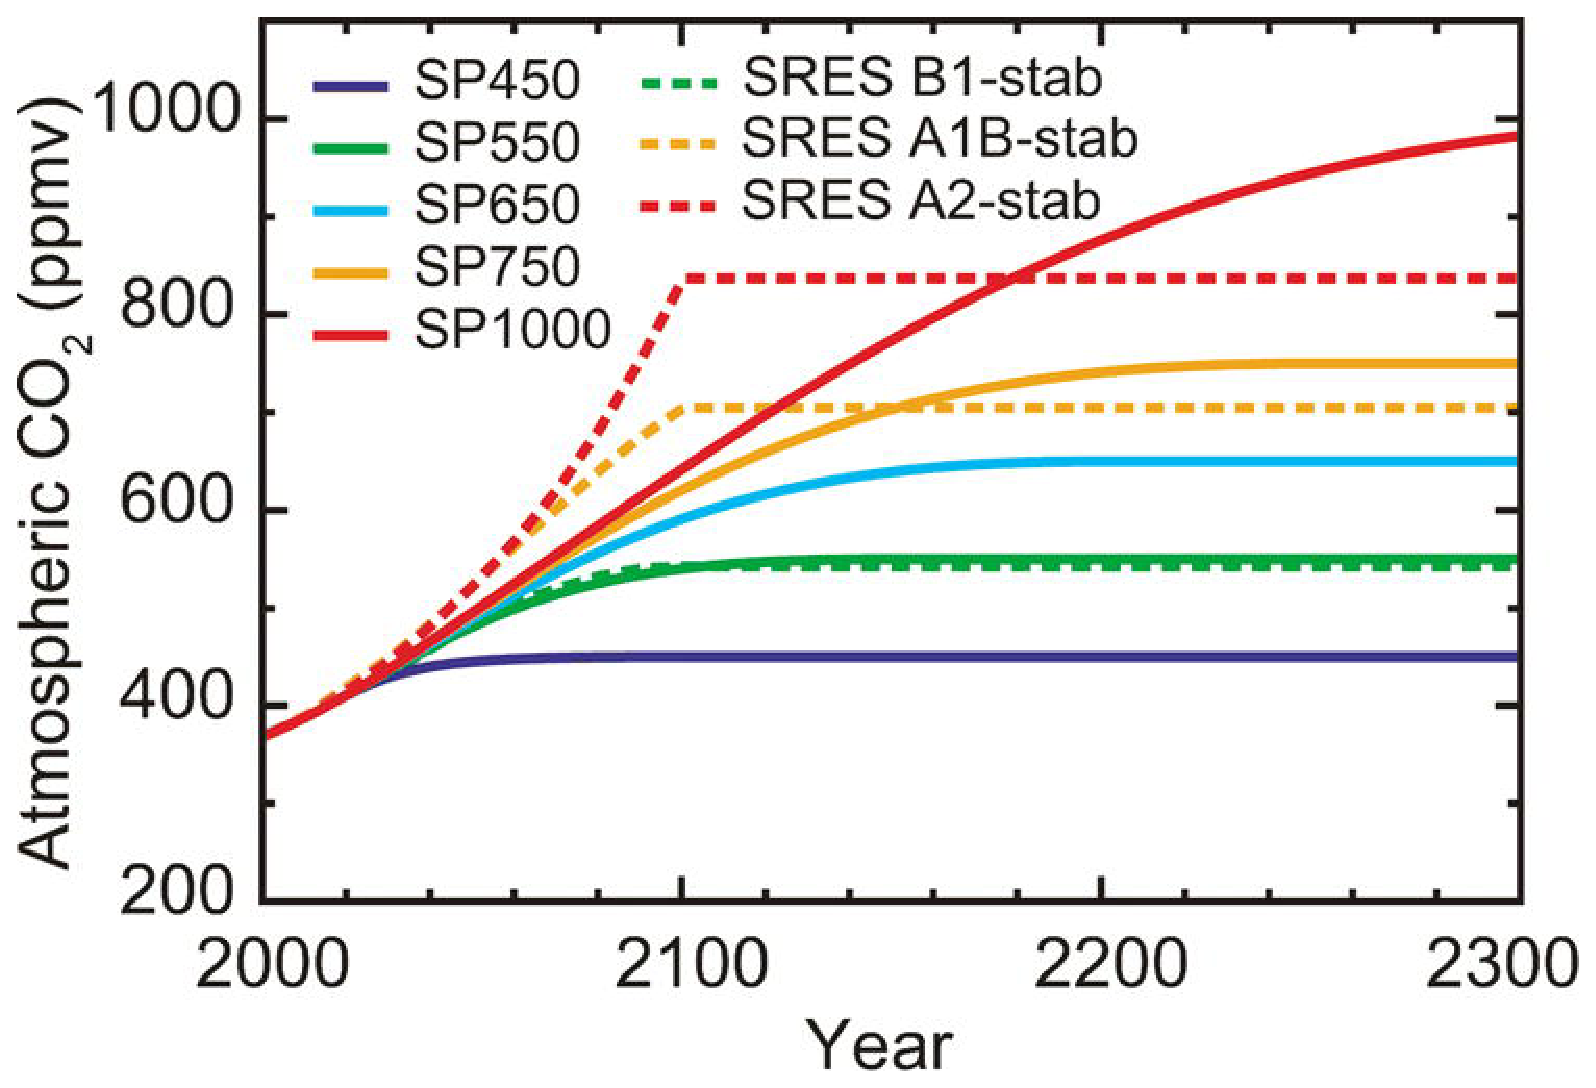
\includegraphics[width=19pc,angle=0]{./figures/figure01.eps}}
\caption{Enter the caption for your figure here.  Repeat as
  necessary for each of your figures. Create a figures directory and
  place all figures in that directory.}\label{fig:02}
\end{figure}

\section{Results}

Text Text Text Text Text Text  Text Text Text Text Text Text Text Text Text  Text Text Text Text Text Text. \textbf{Figure\ref{fig:02}} shows that the above method  Text Text Text Text  Text Text Text Text Text Text  Text Text.  \citealp{Boffelli03} might want to know about  text text text text
Text Text Text Text Text Text  Text Text Text Text Text Text Text Text Text  Text Text Text Text Text Text. \textbf{Figure\ref{fig:02}} shows that the above method  Text Text Text Text  Text Text Text Text Text Text  Text Text.  \citealp{Boffelli03} might want to know about  text text text text
Text Text Text Text Text Text  Text Text Text Text.


\textbf{Table\ref{Tab:01}} shows that Text Text Text Text Text  Text Text Text Text Text Text. \textbf{Figure\ref{fig:02}} shows that
the above method Text Text. Text Text Text  Text Text Text Text Text Text. \textbf{Figure\ref{fig:02}} shows that
the above method Text Text. Text Text Text  Text Text Text Text Text Text. \textbf{Figure\ref{fig:02}} shows that
the above method Text Text. For more information, check out the {website$^{}$}\footnote{\url{http://www.math.uiuc.edu/~hildebr/tex}}


\section{Discussion}

(\textbf{Table\ref{Tab:01}}) Text Text Text Text Text Text  Text Text Text Text Text Text Text Text Text  Text Text Text Text Text Text. \textbf{Figure\ref{fig:02}} shows that the above method  Text Text Text Text  Text Text Text Text Text Text  Text Text.  \citealp{Boffelli03} might want to know about  text text text text
Text Text Text Text Text Text  Text Text Text Text Text Text Text Text Text  Text Text Text Text Text Text. \textbf{Figure\ref{fig:02}} shows that the above method  Text Text Text Text  Text Text Text Text Text Text  Text Text.  \citealp{Boffelli03} might want to know about  text text text text
Text Text Text Text Text Text  Text Text Text Text Text Text Text Text Text  Text Text Text Text Text Text. \textbf{Figure\ref{fig:02}} shows that the above method  Text Text Text Text  Text Text Text Text Text Text  Text Text. 


Text Text Text Text Text Text  Text Text Text Text Text Text Text Text Text  Text Text Text Text Text Text. \textbf{Figure\ref{fig:02}} shows that the above method  Text Text Text Text  Text Text Text Text Text Text  Text Text.  \citealp{Boffelli03} might want to know about  text text text text

\begin{enumerate}
\item this is item, use enumerate
\item this is item, use enumerate
\item this is item, use enumerate
\end{enumerate}

Text Text Text Text Text Text  Text Text Text Text Text Text Text Text Text  Text Text Text Text Text Text. \textbf{Figure\ref{fig:02}} shows that the above method  Text Text Text Text  Text Text Text Text Text Text  Text Text.  \citealp{Boffelli03} might want to know about  text text text text
Text Text Text Text Text Text  Text Text Text Text Text Text Text Text Text  Text Text Text Text Text Text. \textbf{Figure\ref{fig:02}} shows that the above method  Text Text Text Text  Text Text Text Text Text Text  Text Text.  \citealp{Boffelli03} might want to know about  text text text text
Text Text Text Text Text Text  Text Text Text Text Text Text Text Text Text  Text Text Text Text Text Text.

Text Text Text Text Text Text  Text Text Text Text Text Text Text Text Text  Text Text Text Text Text Text. \textbf{Figure\ref{fig:02}} shows that the above method  Text Text Text Text

\section*{Disclosure/Conflict-of-Interest Statement}
Text Text Text Text Text Text  Text Text Text Text Text Text Text Text  Text Text Text Text Text Text Text Text Text  Text Text Text.

\section*{Acknowledgement}
Text Text Text Text Text Text  Text Text Text Text Text Text Text Text  Text Text Text Text Text Text Text Text Text  Text Text Text.  

\paragraph{Funding\textcolon} Text Text Text Text Text Text  Text Text.

\section*{Supplemental Data}
Text Text Text Text Text Text  Text Text Text Text Text Text Text Text Text  Text Text Text Text Text Text Text Text Text  Text Text Text.

%\bibliographystyle{natbib}
%\bibliographystyle{achemnat}
%\bibliographystyle{plainnat}
%\bibliographystyle{abbrv}
%\bibliographystyle{bioinformatics}
%
%\bibliographystyle{plain}
%
%\bibliography{Document}


\begin{thebibliography}{}
\bibitem[Bofelli {et~al}., 2000]{Boffelli03} Bofelli,F., Name2, Name3 (2003) Article title, {\it Journal Name}, {\bf 199}, 133-154.

\bibitem[Bag {et~al}., 2001]{Bag01} Bag,M., Name2, Name3 (2001) Article title, {\it Journal Name}, {\bf 99}, 33-54.

\bibitem[Yoo {et~al}., 2003]{Yoo03}
Yoo,M.S. {et~al}. (2003) Oxidative stress regulated genes
in nigral dopaminergic neurnol cell: correlation with the known
pathology in Parkinson's disease. \textit{Brain Res. Mol. Brain
Res.}, \textbf{110}(Suppl. 1), 76--84.

\bibitem[Lehmann, 1986]{Leh86}
Lehmann,E.L. (1986) Chapter title. \textit{Book Title}. Vol.~1, 2nd edn. Springer-Verlag, New York, pp.???--???.

\bibitem[Crenshaw and Jones, 2003]{Cre03}
Crenshaw, B.,III, and Jones, W.B.,Jr (2003) The future of clinical
cancer management: one tumor, one chip. \textit{Bioinformatics},
doi:10.1093/bioinformatics/btn000.

\bibitem[Auhtor {et~al}. (2000)]{Aut00}
Auhtor,A.B. {et~al}. (2000) Chapter title. In Smith, A.C.
(ed.), \textit{Book Title}, 2nd edn. Publisher, Location, Vol. 1, pp.
???--???.

\bibitem[Bardet, 1920]{Bar20}
Bardet, G. (1920) Sur un syndrome d'obesite infantile avec
polydactylie et retinite pigmentaire (contribution a l'etude des
formes cliniques de l'obesite hypophysaire). PhD Thesis, name of
institution, Paris, France.

\end{thebibliography}
\end{document}
